\chapter{Results}
\label{sec:results}

\section{Charging without photoemission}

\section{Charging with photoemission}

\subsection*{Drift parallel to X axis}

%FLOATING POTENTIAL CONVERGENCE
\begin{center}
    \begin{figure}[H]
      \begin{subfigure}[b]{0.75\textwidth}
      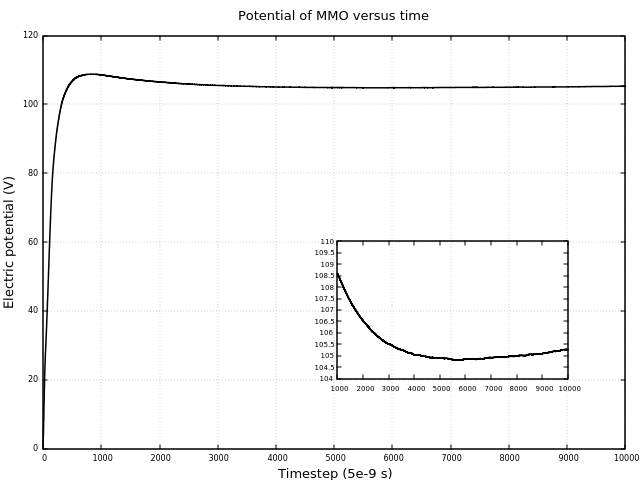
\includegraphics[width=\columnwidth]{figures/MMO/plusX/Booms/MMO_Booms_driftplusX_timeseries.png}
      \caption{Booms}
      \label{fig:MMO_Booms_driftplusX_timeseries}
    \end{subfigure}
    \par\bigskip
    \begin{subfigure}[b]{0.75\textwidth}
      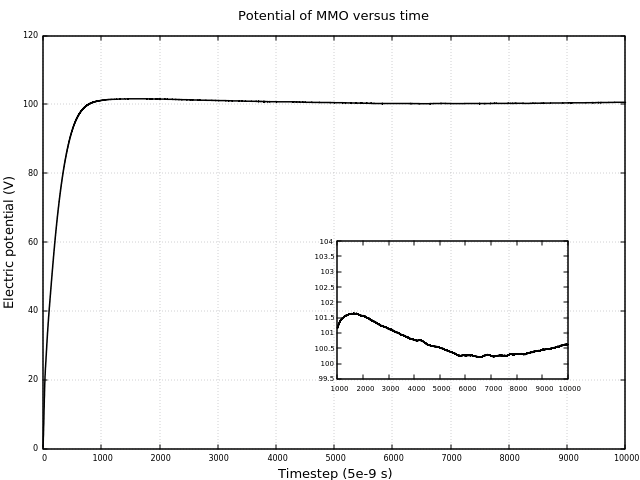
\includegraphics[width=\columnwidth]{figures/MMO/plusX/noBooms/MMO_noBooms_driftplusX_timeseries.png}
      \caption{Without booms}
      \label{fig:MMO_noBooms_driftplusX_timeseries}
    \end{subfigure}
  \label{fig:DriftPlusXTimeseries}
  \caption{Time series plot of the potential of the MMO with and without booms. The inset plots the same timeseries after 1000 timesteps, where the potential of the spacecraft has begun to oscillate about the floating potential.}
  \end{figure}
\end{center}


%POTENTIAL THROUGH CENTER OF OBJECT
\begin{center}
    \begin{figure}[H]
      \begin{subfigure}[b]{0.61\textwidth}
      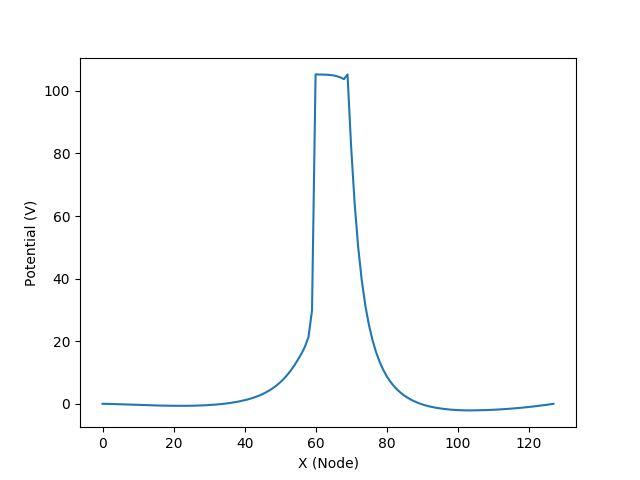
\includegraphics[width=\textwidth]{figures/MMO/plusX/Booms/PhiXBoomsPlusX.png}
      \caption{Booms}
      \label{fig:PhiXBoomsPlusX}
    \end{subfigure}
    \begin{subfigure}[b]{0.61\textwidth}
      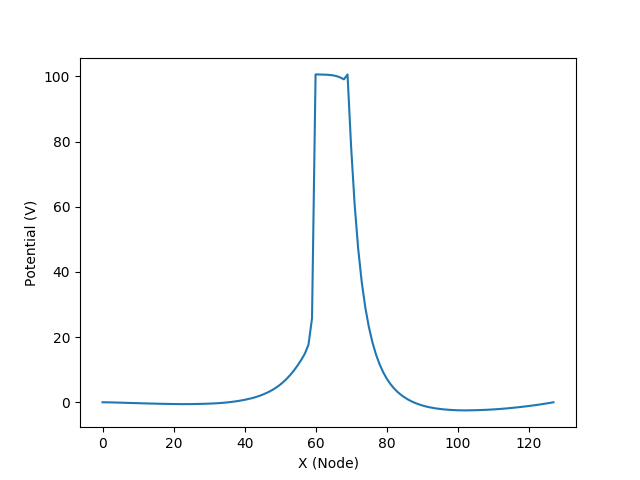
\includegraphics[width=\textwidth]{figures/MMO/plusX/noBooms/PhiXnoBoomsPlusX.png}
      \caption{Without booms}
      \label{fig:PhiXnoBoomsPlusX}
    \end{subfigure}
  \label{fig:PhiXDriftX}
  \caption{Dummy text}
  \end{figure}
\end{center}


%PARTICLE DENSITIES (rho_i and rho_e)
%RHO_I
\begin{comment}
\begin{center}
    \begin{figure}[H]
      \begin{subfigure}[b]{0.61\textwidth}
      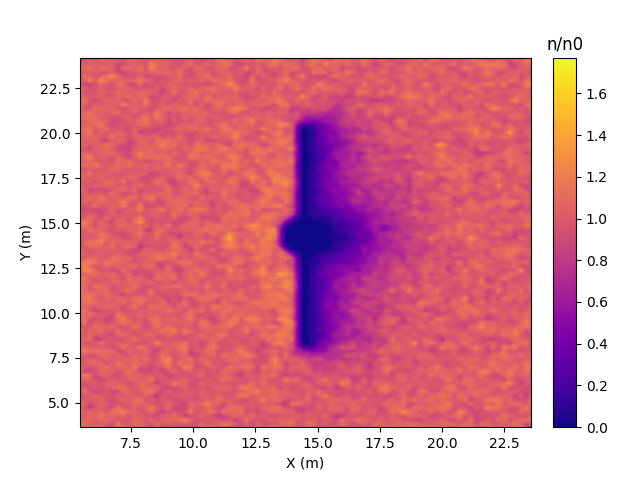
\includegraphics[width=\textwidth]{figures/MMO/plusX/Booms/BoomsPlusXrhoIT5000.png}
      \caption{Booms}
      \label{fig:PhiXBoomsPlusX}
    \end{subfigure}
    \begin{subfigure}[b]{0.61\textwidth}
      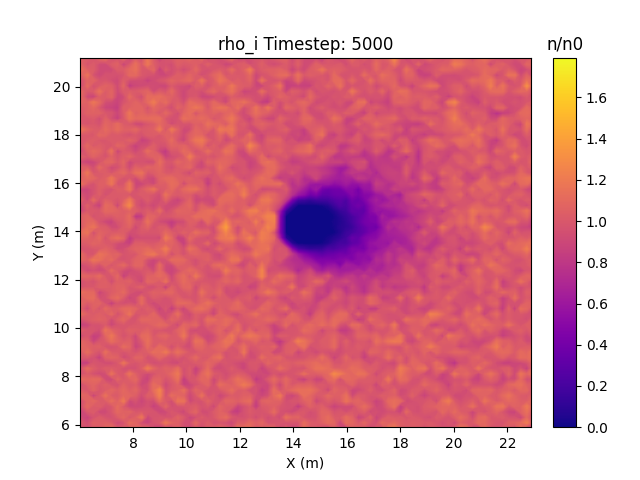
\includegraphics[width=\textwidth]{figures/MMO/plusX/noBooms/noBoomsPlusXrhoIT5000.png}
      \caption{Without booms}
      \label{fig:PhiXnoBoomsPlusX}
    \end{subfigure}
  \label{fig:PhiXDriftX}
  \caption{Dummy text}
  \end{figure}
\end{center}

%RHO_E
\begin{center}
    \begin{figure}[H]
      \begin{subfigure}[b]{0.61\textwidth}
      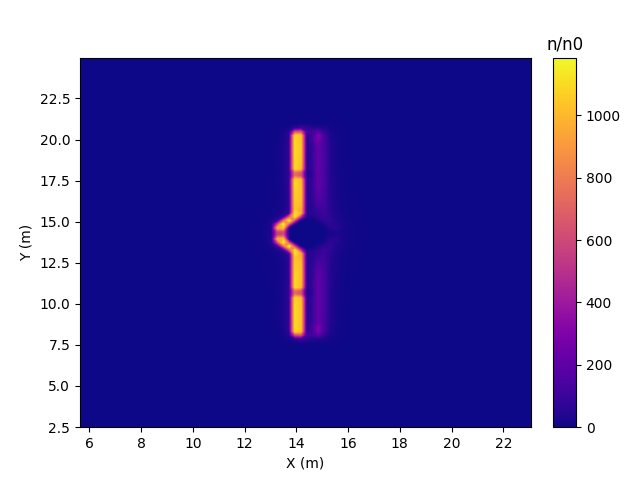
\includegraphics[width=\textwidth]{figures/MMO/plusX/Booms/BoomsPlusXrhoET5000.png}
      \caption{Booms}
      \label{fig:PhiXBoomsPlusX}
    \end{subfigure}
    \begin{subfigure}[b]{0.61\textwidth}
      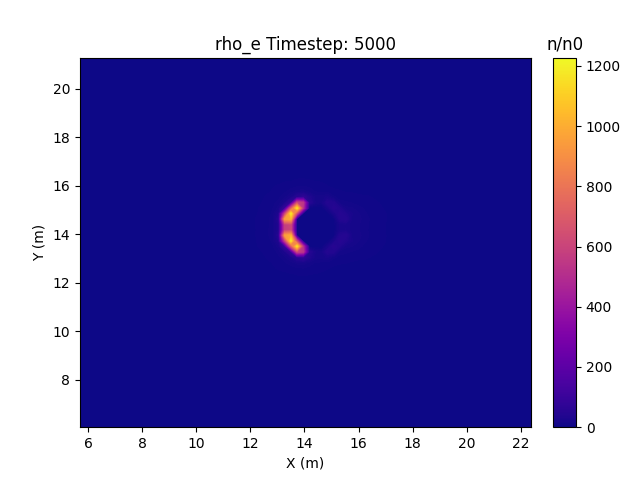
\includegraphics[width=\textwidth]{figures/MMO/plusX/noBooms/noBoomsPlusXrhoET5000.png}
      \caption{Without booms}
      \label{fig:PhiXnoBoomsPlusX}
    \end{subfigure}
  \label{fig:PhiXDriftX}
  \caption{Dummy text}
  \end{figure}
\end{center}
\end{comment}



%AVERAGE POTENTIAL ISOLINES XY
\begin{center}
\begin{figure}[H]
  \begin{subfigure}[b]{0.61\textwidth}
    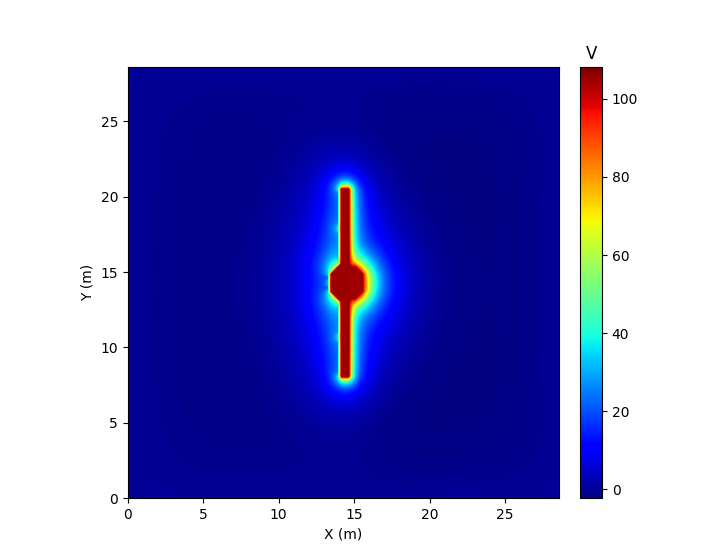
\includegraphics[width=\textwidth]{figures/MMO/plusX/Booms/AvgAfter1000BoomsPlusX.png}
    \caption{Booms}
    \label{fig:AvgAfter1000BoomsPlusX}
  \end{subfigure}
  \hfill
  \begin{subfigure}[b]{0.61\textwidth}
    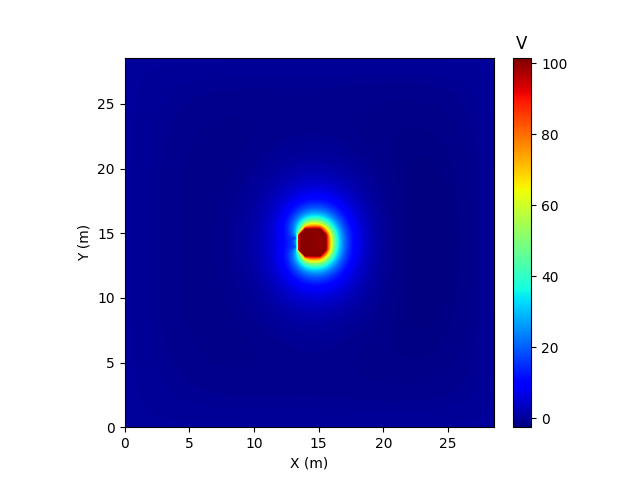
\includegraphics[width=\textwidth]{figures/MMO/plusX/noBooms/AvgAfter1000noBoomsPlusX.png}
    \caption{Without booms}
    \label{fig:AvgAfter1000noBoomsPlusX}
  \end{subfigure}
  \label{fig:AvgPhiDriftX}
  \caption{Dummy text}
\end{figure}
\end{center}



\subsection*{Drift parallel to Z axis}


%PARTICLE DENSITIES (rho_i and rho_e)
%RHO_I
\begin{comment}
\begin{center}
    \begin{figure}[H]
      \begin{subfigure}[b]{0.61\textwidth}
      \includegraphics[width=\textwidth]{}
      \caption{Booms}
      \label{fig:PhiXBoomsPlusX}
    \end{subfigure}
    \begin{subfigure}[b]{0.61\textwidth}
      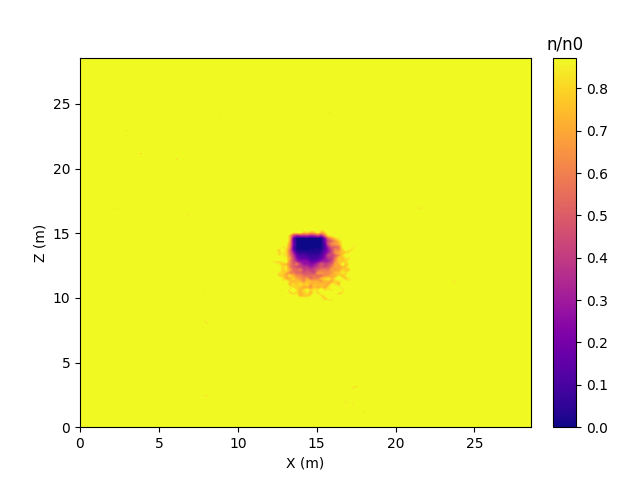
\includegraphics[width=\textwidth]{figures/MMO/minZ/noBooms/noBoomMinZrhoIT5000XZRestr05.png}
      \caption{Without booms}
      \label{fig:PhiXnoBoomsPlusX}
    \end{subfigure}
  \label{fig:PhiXDriftX}
  \caption{Dummy text}
  \end{figure}
\end{center}

\begin{center}
    \begin{figure}[H]
      \begin{subfigure}[b]{0.61\textwidth}
      \includegraphics[width=\textwidth]{}
      \caption{Booms}
      \label{fig:PhiXBoomsPlusX}
    \end{subfigure}
    \begin{subfigure}[b]{0.61\textwidth}
      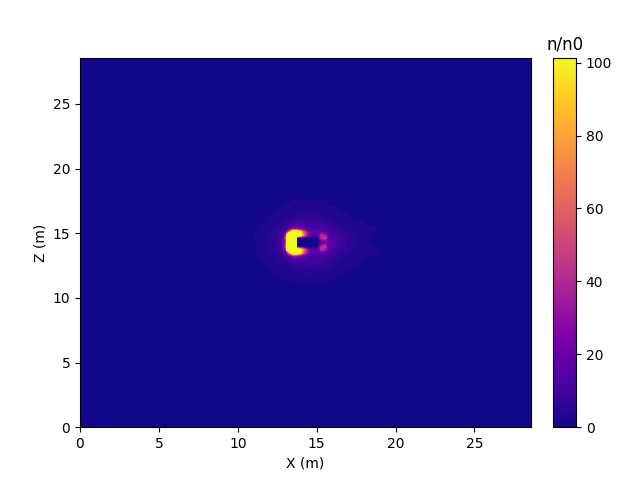
\includegraphics[width=\textwidth]{figures/MMO/minZ/noBooms/noBoomMinZrhoET5000XZRestr01.png}
      \caption{Without booms}
      \label{fig:PhiXnoBoomsPlusX}
    \end{subfigure}
  \label{fig:PhiXDriftX}
  \caption{Dummy text}
  \end{figure}
\end{center}
\end{comment}


\section{Charging in an external magnetic field}







\section{Charging at different photoelectron temperatures}